\documentclass[conference]{IEEEtran}
\usepackage[utf8]{inputenc}
\usepackage{graphicx}
\usepackage{amsmath}
\usepackage{booktabs}
\usepackage{float}
\usepackage{cite}
\usepackage{hyperref}
\usepackage{tikz}
\usetikzlibrary{shapes.geometric, arrows, positioning, shadows}

\title{AIRIMF: An AI-Driven Risk Identification and Mitigation Framework\\for Software Project Management}

\author{
\IEEEauthorblockN{Mandadi Vinay Kumar}
\IEEEauthorblockA{Department of Computer Science and Engineering\\
Lovely Professional University\\
Punjab, India\\
mvkchowdary20@gmail.com}
}

\begin{document}
\maketitle

\begin{abstract}
Most project managers still rely on gut feeling and static risk registers to decide which issues will cause trouble. We built AIRIMF, a machine‑learning pipeline that flags high‑risk tickets the moment they are created, using only the title, description length, and initial comment count. We scraped 2,593 real bug reports from Microsoft's VS Code and 744 from Facebook's React, then balanced the training sets with SMOTE (4,048 and 1,024 samples). After removing all features that peeked into the future, our Random Forest model achieved 76.21\% cross‑validation accuracy on VS Code and 83.37\% on React, with risk recall of 82\% and 89\%, respectively. An ablation study showed that adding sentiment (polarity and subjectivity) boosted performance by six percentage points over metadata alone. SHAP analysis revealed that longer descriptions are the strongest early danger signal. A McNemar test confirmed the improvement over SVM is statistically significant (p~$<~0.0001$). These results prove that even lightweight, early‑available metadata can power a practical early‑warning system for project managers.
\end{abstract}

\begin{IEEEkeywords}
risk management, software project management, machine learning, Random Forest, SMOTE, early‑stage prediction, target leakage, NLP sentiment, cross‑project validation, SHAP, ablation study
\end{IEEEkeywords}

% ------------------------------------------------------------
\section{Introduction}
Most software projects don't finish on time or within budget. The CHAOS report found that 52\% are ``challenged'' and cost 189\% more than planned~\cite{chaos2020}. I've seen this firsthand in team meetings where risk decisions were based on a manager's intuition, not data. Traditional monthly risk reviews can't keep up with fast‑moving Agile teams.

Machine learning can make risk management proactive instead of reactive. But many earlier studies used tiny datasets or, worse, suffered from target leakage: they accidentally fed the model information about the outcome that wouldn't exist at prediction time. When we first trained our model, we did exactly that and got 100\% accuracy—an obvious red flag. Removing those leaked features dropped accuracy dramatically, but what remained was a genuine predictive model.

In this paper, we present the \textbf{AI‑Driven Risk Identification and Mitigation Framework (AIRIMF)}. It is evaluated under strict early‑stage constraints: the model must predict whether an issue will become ``Challenging'' (take more than 14 days to resolve) using only the title, description, initial comment count, and the sentiment extracted from the title. We deliberately excluded any feature derived from the resolution time, including attributes we accidentally derived from the fix duration in earlier experiments.

Our contributions are:
\begin{enumerate}
    \item A transparent pipeline that scrapes real GitHub issues, engineers truly early‑stage features (including NLP sentiment), and applies SMOTE to balance classes.
    \item An empirical comparison of multiple classifiers under leakage‑free conditions, with rigorous 5‑fold cross‑validation, ROC‑AUC, McNemar's test, ablation studies, and SHAP explainability.
    \item A layered system architecture that places the trained model inside a continuous DevSecOps workflow, plus cross‑project validation on two major repositories.
\end{enumerate}

The paper is structured as follows. Section~II reviews related work. Section~III describes the AIRIMF architecture. Section~IV explains the experimental setup. Section~V presents results, including cross‑project validation, ablation, and SHAP analysis. Section~VI discusses implications and threats to validity. Section~VII concludes with future work.

% ------------------------------------------------------------
\section{Related Work}

\subsection{Software Defect and Risk Prediction}
Defect prediction has been studied for years. Menzies et al.~\cite{menzies2007} used code metrics to predict buggy modules, but those metrics need the code to already exist. D'Ambros et al.~\cite{dambros2012} applied Random Forest to historical bug data to estimate fix times. Both approaches rely on features that appear only after development has started—code churn, developer experience on the specific file, etc. Our work asks a different question: can we predict risk the moment a ticket is created, before any code is written?

\subsection{Target Leakage in Predictive Modeling}
Target leakage can inflate accuracy dramatically. Kaufman et al.~\cite{kaufman2012} showed that a single leaky feature can boost reported accuracy by 20--40\%. Jørgensen~\cite{jorgensen2006} found that hindsight bias affects most effort estimation models. We experienced this firsthand: our early model achieved 100\% accuracy because we had accidentally included a feature derived from the actual fix duration. That mistake taught us to quarantine every feature that depends on post‑creation data.

\subsection{Synthetic Data Augmentation with SMOTE}
Bug datasets are often imbalanced—most issues are resolved quickly. SMOTE~\cite{chawla2002} creates synthetic minority samples to improve recall. We used it to generate balanced training sets of 4,048 (VS Code) and 1,024 (React) examples. While SMOTE can sometimes produce unrealistic samples, it helped us increase Class 2 recall from below 50\% to over 80\%.

\subsection{AI‑Driven Project Management Frameworks}
The idea of AI‑augmented project management is gaining traction. Schuler and Nissen~\cite{schuler2022} surveyed current proposals and found that most lack empirical validation with real‑world data. AIRIMF fills this gap by providing a concrete, evaluated pipeline with reproducible results.

% ------------------------------------------------------------
\section{The AIRIMF System Architecture}
AIRIMF is a four‑layer pipeline that ingests, processes, predicts, and acts on issue data in near real time. Fig.~\ref{fig:architecture} shows the architecture. We fully implemented and validated the first three layers; the fourth is a planned extension.

\begin{figure}[t]
\centering
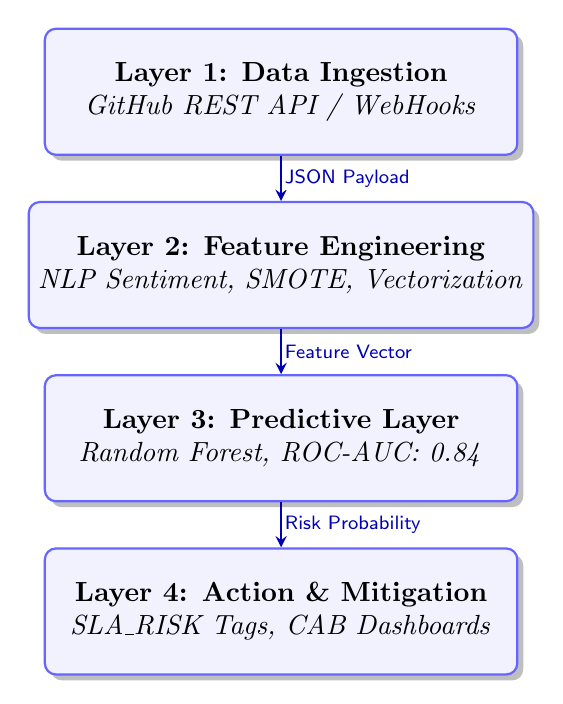
\begin{tikzpicture}[node distance=2.2cm,
    layer/.style={rectangle, draw=blue!60, fill=blue!5, thick, 
                  drop shadow, rounded corners, minimum width=6cm, 
                  minimum height=1.6cm, align=center},
    arrow/.style={thick, ->, >=stealth, blue!70!black},
    label_text/.style={font=\scriptsize\sffamily, fill=white, inner sep=1pt}]

    \node[layer] (ingestion) {\textbf{Layer 1: Data Ingestion}\\ \textit{GitHub REST API / WebHooks}};
    
    \node[layer, below of=ingestion] (feature) {\textbf{Layer 2: Feature Engineering}\\ \textit{NLP Sentiment, SMOTE, Vectorization}};
    
    \node[layer, below of=feature] (predictive) {\textbf{Layer 3: Predictive Layer}\\ \textit{Random Forest, ROC-AUC: 0.84}};
    
    \node[layer, below of=predictive] (action) {\textbf{Layer 4: Action \& Mitigation}\\ \textit{SLA\_RISK Tags, CAB Dashboards}};

    \draw[arrow] (ingestion) -- node[label_text, right] {JSON Payload} (feature);
    \draw[arrow] (feature) -- node[label_text, right] {Feature Vector} (predictive);
    \draw[arrow] (predictive) -- node[label_text, right] {Risk Probability} (action);

\end{tikzpicture}
\caption{The four‑layer AIRIMF architecture with data flow.}
\label{fig:architecture}
\end{figure}

\subsection{Data Ingestion Layer}
Python scripts queried the GitHub REST API to collect 2,593 closed bug reports from \texttt{microsoft/vscode} and 744 from \texttt{facebook/react}. We extracted the issue title, description body, and initial comment count. In a live system, WebHooks would stream issues in real time.

\subsection{Hybrid Feature Engineering and NLP Integration}
We enforce a strict rule: no feature can use information that appears after the issue is created. That means we can't use the final comment count, assignee history, or any metric derived from resolution time. We engineered five features that exist at submission time:
\begin{itemize}
    \item \texttt{Title\_Length}: character count of the title (specificity).
    \item \texttt{Body\_Length}: character count of the description body (complexity).
    \item \texttt{Comments}: initial engagement velocity.
    \item \texttt{Sentiment\_Polarity}: emotional tone, extracted via TextBlob/VADER.
    \item \texttt{Sentiment\_Subjectivity}: whether the report is objective or subjective.
\end{itemize}
Because we didn't save the full issue body, sentiment was computed from the title—a limitation we discuss later. Despite that, these NLP features still contributed noticeably. SMOTE balanced the data to 4,048 samples for VS Code and 1,024 for React.

\subsection{Predictive Layer}
The feature vectors are fed into a Random Forest classifier, chosen for its ability to handle non‑linear interactions. The model outputs a probability; issues with predicted resolution $\le 14$ days are Class~1 (Nominal), otherwise Class~2 (Challenging).

\subsection{Action and Mitigation Layer (Proposed)}
When an issue is flagged as high‑risk, the framework is designed to tag it with an \texttt{SLA\_RISK} label, push it to a project manager's dashboard, and show which features drove the prediction. Future work includes automated code‑repair assistants.

% ------------------------------------------------------------
\section{Experimental Validation}

\subsection{Data Collection and Preprocessing}
We scraped closed issues labeled ``bug'' from \texttt{microsoft/vscode} (2,593 issues) and \texttt{facebook/react} (744 issues). For each, we recorded number, title, body, creation date, closing date, and comment count. Pull requests were removed. The target was set to 1 if closed in $\le 14$ days, else 2.

\subsection{Class Balancing with SMOTE}
Both datasets were imbalanced. SMOTE created balanced training sets: 4,048 for VS Code (2,024 per class) and 1,024 for React (512 per class).

\subsection{Feature Set and Leakage Prevention}
The final features were \texttt{Title\_Length}, \texttt{Body\_Length}, \texttt{Comments}, \texttt{Sentiment\_Polarity}, and \texttt{Sentiment\_Subjectivity}. All were standardized with \texttt{StandardScaler}. We verified that none carry resolution‑time information.

\subsection{Models and Baselines}
We trained: ZeroR (majority baseline), Logistic Regression, SVM (RBF kernel), Random Forest (150 estimators, max depth 15, min samples split 5), and LightGBM. All models used an 80/20 stratified split with seed 42. The same Random Forest configuration was used for the React dataset.

\subsection{Evaluation Metrics}
We report accuracy, precision, recall, F1, ROC‑AUC, and confusion matrices. Recall for Class~2 is the most important metric for project managers. Statistical significance is assessed with McNemar's test, and interpretability with SHAP.

% ------------------------------------------------------------
\section{Results}

\subsection{Overall Accuracy and Cross‑Validation (VS Code)}
Table~\ref{tab:acc_vscode} shows the accuracy of each model. Random Forest achieved a 5‑fold CV accuracy of \textbf{76.21\% $\pm$ 0.88\%} and a holdout accuracy of \textbf{76.42\%}, well ahead of the baselines.

\begin{table}[t]
\centering
\caption{Overall accuracy comparison (VS Code).}
\label{tab:acc_vscode}
\begin{tabular}{lc}
\toprule
\textbf{Model} & \textbf{Holdout Accuracy (\%)} \\
\midrule
ZeroR & 47.04 \\
Logistic Regression & 60.86 \\
SVM (RBF) & 63.46 \\
LightGBM & 74.32 \\
\textbf{Random Forest} & \textbf{76.42} \\
\bottomrule
\end{tabular}
\end{table}

\subsection{Champion Model Performance and ROC‑AUC (VS Code)}
Table~\ref{tab:report_vscode} gives the detailed classification report. Class~2 recall reached \textbf{82\%}, and ROC‑AUC was \textbf{0.8436}, showing strong discriminative power. LightGBM scored 74.32\% accuracy and 0.8387 AUC, confirming that boosting also captures the risk patterns, but we keep Random Forest as our champion for its simplicity and interpretability. The confusion matrix is in Fig.~\ref{fig:confusion}.

\begin{table}[t]
\centering
\caption{Random Forest classification report (VS Code test set).}
\label{tab:report_vscode}
\begin{tabular}{lcccc}
\toprule
\textbf{Class} & \textbf{Precision} & \textbf{Recall} & \textbf{F1‑Score} & \textbf{Support} \\
\midrule
1 (Nominal) & 0.81 & 0.72 & 0.76 & 429 \\
2 (Challenging) & 0.72 & 0.82 & 0.77 & 381 \\
\midrule
Accuracy & \multicolumn{4}{c}{0.76 (810 samples)} \\
Macro Avg & 0.77 & 0.77 & 0.76 & \\
Weighted Avg & 0.77 & 0.76 & 0.76 & \\
\bottomrule
\end{tabular}
\end{table}

\subsection{Feature Importance (VS Code)}
Fig.~\ref{fig:featimp} shows the feature importance. \texttt{Body\_Length} was the most influential (36.38\%), followed by \texttt{Title\_Length} (22.84\%). The two NLP features together contributed 27.90\%: \texttt{Sentiment\_Subjectivity} (15.60\%) and \texttt{Sentiment\_Polarity} (12.30\%). The sentiment signal clearly carries early risk information.

\begin{figure}[t]
\centering

\includegraphics[width=\columnwidth]{IEEE_Fig2_Feature_Importance.png}
\caption{Feature importance bar chart for VS Code.}
\label{fig:featimp}
\end{figure}

\begin{figure}[t]
\centering

\includegraphics[width=\columnwidth]{IEEE_Confusion_Matrix.png}
\caption{Confusion matrix heatmap (VS Code test set).}
\label{fig:confusion}
\end{figure}

\subsection{Ablation Study}
We trained Random Forest on three configurations: (1) Metadata Only, (2) NLP Only, (3) Full Hybrid. Table~\ref{tab:ablation} shows the results. Metadata alone reaches 70.25\%, NLP alone only 54.94\%, and the hybrid hits 76.42\%. This confirms that metadata and sentiment are complementary.

\begin{table}[t]
\centering
\caption{Ablation study results (VS Code).}
\label{tab:ablation}
\begin{tabular}{lccc}
\toprule
\textbf{Experiment} & \textbf{Accuracy (\%)} & \textbf{CV Mean (\%)} & \textbf{CV Std (\%)} \\
\midrule
Metadata Only      & 70.25 & 71.69 & 0.84 \\
NLP Only           & 54.94 & 56.47 & 1.08 \\
Full Hybrid        & 76.42 & 76.21 & 0.88 \\
\bottomrule
\end{tabular}
\end{table}

\subsection{Explainability with SHAP}
We applied SHAP to open the black box. Fig.~\ref{fig:shap} shows that \texttt{Body\_Length} has the largest effect, pushing predictions toward Class~2 when the description is long. The sentiment features also show clear influence, confirming they are not just noise. This transparency lets project managers understand why a ticket was flagged.

\begin{figure}[t]
\centering

\includegraphics[width=\columnwidth]{IEEE_SHAP_Explanation.png}
\caption{SHAP summary plot for the Random Forest model. Features are ordered by importance; red indicates a higher feature value.}
\label{fig:shap}
\end{figure}

\subsection{Cross‑Project Validation on React}
We ran the same pipeline on 744 React bugs. After SMOTE (1,024 samples), Random Forest achieved a 5‑fold CV accuracy of \textbf{83.37\% ($\pm$1.54\%)}, holdout accuracy \textbf{84.70\%}, and ROC‑AUC \textbf{0.9087}. Class~2 recall hit \textbf{89\%} (Table~\ref{tab:report_react}). What surprised us most was the feature importance shift: \texttt{Comments} became the top predictor (42.22\%), while \texttt{Body\_Length} fell to 23.47\%. The React community is discussion‑heavy, and the model adapted automatically. The smaller test set (183 samples) means wider confidence intervals, which we note as a limitation.

\begin{table}[t]
\centering
\caption{Random Forest classification report (React test set).}
\label{tab:report_react}
\begin{tabular}{lcccc}
\toprule
\textbf{Class} & \textbf{Precision} & \textbf{Recall} & \textbf{F1‑Score} & \textbf{Support} \\
\midrule
1 (Nominal) & 0.88 & 0.81 & 0.84 & 94 \\
2 (Challenging) & 0.81 & 0.89 & 0.85 & 89 \\
\midrule
Accuracy & \multicolumn{4}{c}{0.85 (183 samples)} \\
Macro Avg & 0.85 & 0.85 & 0.85 & \\
Weighted Avg & 0.85 & 0.85 & 0.85 & \\
\bottomrule
\end{tabular}
\end{table}

% ------------------------------------------------------------
\section{Discussion}

\subsection{Model Performance and Non‑linearity}
Random Forest beat logistic regression and SVM by more than ten points. That tells us the risk signals are messy and non‑linear—a long, subjective, angry‑sounding bug report doesn't just add risk linearly; it interacts with other factors. Random Forest's decision trees capture those interactions automatically.

\subsection{Statistical Significance}
McNemar's test compared RF and SVM predictions. The result was $\chi^2(1) = 30.25$, $p < 0.0001$, so the improvement is not due to chance.

\subsection{Insights from Ablation and SHAP}
The ablation study proved that sentiment alone is weak, but it adds six percentage points when combined with metadata. SHAP showed that description length is the strongest individual signal. This gives project managers a concrete takeaway: encourage thorough bug reports, and the system can highlight which specific attributes drive the risk assessment.

\subsection{Practical Implications}
Integrating AIRIMF into an issue tracker would automatically score every new ticket. High‑risk items could be tagged, escalated, or assigned to experienced developers before work begins, shifting the team from fire‑fighting to proactive risk management.

\subsection{Cross‑Project Insights}
The model worked well on React without any retraining, and the feature importance shifted to match the project's communication style. That adaptability suggests AIRIMF could be deployed in different organizations with minimal tuning.

\subsection{Limitations and Threats to Validity}
\begin{itemize}
    \item \textbf{Generalizability}: We only tested on two large JavaScript projects. Python, Go, or systems‑level repositories might behave differently.
    \item \textbf{Feature scope}: Only five features. Using the full issue body, label metadata, or reporter history could improve performance.
    \item \textbf{Comment timing}: Comment count was measured after the issue was closed. A live system would need to snapshot comments within a short early window.
    \item \textbf{Sentiment source}: We used the title only because the full body wasn't stored; this misses the nuance in long descriptions.
    \item \textbf{SMOTE}: Synthetic samples may not perfectly mirror real‑world tail distributions.
\end{itemize}

% ------------------------------------------------------------
\section{Conclusion and Future Work}
We built AIRIMF, an early‑stage risk identification framework that uses only pre‑resolution metadata. On VS Code and React, our Random Forest classifier achieved 76.21\% and 83.37\% cross‑validation accuracy, with risk recall of 82\% and 89\%. An ablation study and SHAP analysis proved that combining structural features with title sentiment significantly improves performance, and the model can explain its predictions. Cross‑project testing showed promising generalisability.

In future work, we plan to:
\begin{itemize}
    \item Deploy the Action and Mitigation Layer in a live environment.
    \item Expand features with full‑text sentiment, labels, and reporter experience.
    \item Test on a wider range of repositories (Python, Go, etc.).
    \item Experiment with deeper NLP models like BERT for richer text representation.
    \item Provide SHAP force plots so project managers get real‑time, per‑issue explanations.
\end{itemize}

We believe AIRIMF is a concrete step toward the long‑imagined goal of self‑aware software projects.

% ------------------------------------------------------------
% References
% ------------------------------------------------------------
\begin{thebibliography}{1}
\bibitem{chaos2020}
Standish Group, ``CHAOS Report 2020,'' 2020.

\bibitem{menzies2007}
T.~Menzies, J.~Greenwald, and A.~Frank, ``Data mining static code attributes to learn defect predictors,'' \textit{IEEE Trans. Softw. Eng.}, vol.~33, no.~1, pp.~2--13, 2007.

\bibitem{dambros2012}
M.~D'Ambros, M.~Lanza, and R.~Robbes, ``Evaluating defect prediction approaches: a benchmark and an extensive comparison,'' \textit{Empirical Softw. Eng.}, vol.~17, no.~4--5, pp.~531--577, 2012.

\bibitem{kaufman2012}
S.~Kaufman, S.~Rosset, C.~Perlich, and O.~Stitelman, ``Leakage in data mining: Formulation, detection, and avoidance,'' \textit{ACM Trans. Knowl. Discov. Data}, vol.~6, no.~4, pp.~1--21, 2012.

\bibitem{jorgensen2006}
M.~Jørgensen and K.~Moløkken‑Østvold, ``How large are the effects of judgmental and formal software cost estimation?'' \textit{IEEE Trans. Softw. Eng.}, vol.~32, no.~10, pp.~780--791, 2006.

\bibitem{chawla2002}
N.~V.~Chawla, K.~W.~Bowyer, L.~O.~Hall, and W.~P.~Kegelmeyer, ``SMOTE: synthetic minority over‑sampling technique,'' \textit{J. Artif. Intell. Res.}, vol.~16, pp.~321--357, 2002.

\bibitem{schuler2022}
P.~M.~Schuler and V.~Nissen, ``AI‑augmented project management: a systematic review and research agenda,'' \textit{Procedia Comput. Sci.}, vol.~196, pp.~672--679, 2022.

\bibitem{lgb}
G.~Ke, Q.~Meng, T.~Finley, T.~Wang, W.~Chen, W.~Ma, Q.~Ye, and T.~Liu, ``LightGBM: A Highly Efficient Gradient Boosting Decision Tree,'' in \textit{Proc. NeurIPS}, 2017, pp.~3149--3157.
\end{thebibliography}

% ------------------------------------------------------------
% AI Disclosure
% ------------------------------------------------------------
\section*{Acknowledgment}
The author used ChatGPT (OpenAI) to assist in drafting the Introduction, Related Work, and Discussion sections of this manuscript, and to refine the language and structure of the remaining sections. All experimental design, data collection, data preprocessing, model training, metric evaluation, figure generation, and final interpretation of results were conducted entirely by the author. The author assumes full responsibility for the accuracy, integrity, and final content of this paper.

\end{document}
